\documentclass[letterpaper]{article}

\usepackage{natbib,alifeconf}  %% The order is important


% *****************
%  Requirements:
% *****************
%
% - All pages sized consistently at 8.5 x 11 inches (US letter size).
% - PDF length <= 8 pages for full papers, <=2 pages for extended
%    abstracts.
% - Abstract length <= 250 words.
% - No visible crop marks.
% - Images at no greater than 300 dpi, scaled at 100%.
% - Embedded open type fonts only.
% - All layers flattened.
% - No attachments.
% - All desired links active in the files.

% Note that the PDF file must not exceed 5 MB if it is to be indexed
% by Google Scholar. Additional information about Google Scholar
% can be found here:
% http://www.google.com/intl/en/scholar/inclusion.html.


% If your system does not generate letter format documents by default,
% you can use the following workflow:
% latex example
% bibtex example
% latex example ; latex example
% dvips -o example.ps -t letterSize example.dvi
% ps2pdf example.ps example.pdf


% For pdflatex users:
% The alifeconf style file loads the "graphicx" package, and
% this may lead some users of pdflatex to experience problems.
% These can be fixed by editing the alifeconf.sty file to specify:
% \usepackage[pdftex]{graphicx}
%   instead of
% \usepackage{graphicx}.
% The PDF output generated by pdflatex should match the required
% specifications and obviously the dvips and ps2pdf steps become
% unnecessary.


% Note:  Some laser printers have a serious problem printing TeX
% output. The use of ps type I fonts should avoid this problem.


\title{Something about lineage metrics}
%\author{Chris Adami$^{1}$, Ryoichi Seki$^{1,2}$ \and Robel Yirdaw$^2$ \\
%\mbox{}\\
%$^1$California Institute of Technology, Pasadena, CA 91125 \\
%$^2$California State University, Northridge, CA 91330 \\
%adami@caltech.edu} % email of corresponding author

% For several authors from the same institution use the same number to
% refer to one address.
%
% If the names do not fit well on one line use
%         Author 1, Author 2 ... \\ {\Large\bf Author n} ...\\ ...
%
% If the title and author information do not fit in the area
% allocated, place \setlength\titlebox{<new height>} after the
% \documentclass line where <new height> is 2.25in



\begin{document}
\maketitle

\begin{abstract}

\end{abstract}

\section{Introduction}

Evolution is an emergent effect of events (\textit{e.g.} replication, variation, and competition) that occur on a much finer-grained temporal scale. While this is a large part of why it is so fascinating, it also presents challenges to studying the short-term mechanisms that govern long-term results. In computational evolutionary systems, we theoretically have adequate data to untangle these mechanisms. In practice, though, gathering appropriate data to do so can be challenging. Moreover, because of the vast difference between the scales that the causes and effects occur on, the quantity of such data can be overwhelming. Both of these problems can be mitigated with a standardized set of diagnostic summary metrics that paint a picture of shorter-term evolutionary dynamics within a population. Here, we introduce a suite of such metrics that operate on lineages and provide an intuition for what they can tell us about evolution.

% Useful suites of metrics in ALIFE?
% - Activity statistics
% - ... 

A lineage describes a continuous line of descent, linking ancestors and their descendants. A complete lineage can provide a post-hoc, step-by-step guide to the evolution of an extant organism where each step involves replication and inherited variation. Indeed, lineage analyses are a powerful tool for disentangling the evolution of complexity in both natural and digital systems; digital systems, however, allow for fine-grained lineage tracking at resolutions that are impossible in modern wet lab experiments, allowing us to replay the tape of life in exacting detail to tease apart the evolutionary recipe for whatever complex feature we happen to be interested in. 
Yet, tracking the full details of a single lineage, much less a population of lineages, can be computationally expensive and will inevitably generate an unwieldy amount of data that can be challenging to visualize and interpret [CITATIONS]. Summary statistics can help alleviate these issues by focusing on general trends(?) for a population rather than for each individual.
% @AML: Need a transition from here to next paragraph about how diagnostic/summary statistics can help
% @SPJ: Something like this?

Here, we demonstrate three types of lineage measurements: lineage length, mutation accumulation, and phenotypic volatility. For each, we discuss their application and our intuitions for what they can tell us about evolution. We evaluate our intuitions on a set of two-dimensional, real-valued optimization problems under a range of mutation rates and selection strengths.   
% @AML: we'll want to say something here about how we talk about how these metrics extend to genetically discrete organisms (e.g. GP)

\section{Metrics}
% Outlining some points to (maybe) make here; probably too bogged down in details; not even sure we want to talk about lineages as graphs:
% - Apply metrics in context of asexual populations
% - Establish a framework from which to think about metrics (not novel, but rarely formalized)
% 	 - We treat lineages as sequences of states where each state represents an individual and transitions between states represent parent-offspring relationships.
%      - More formally, lineages are directed acyclic graphs where internal nodes have in-degree = 1 (parent), out-degree = 1 (offspring). Original ancestor (in digital evolution, often seed of population) w/out-degree = 1. Extant individual w/in-degree = 1.
%      - Transitions specify relevant variation introduced into offspring (e.g. mutations)
%      - States specify relevant genotype and phenotype information (e.g. genome, location in space, behavior, etc) -- anything we might want to measure over a lineage
%      - Becomes more complicated with sexual populations, but we'll stick with asexual assumption for this. 
%  - Already, framework affords certain questions:
%     - How many individuals are along the lineage? 
%     - Total # and magnitude of mutations along lineage?
%     - Distribution of mutation types (ins vs. sub/beneficial vs. deleterious)?
%  - Further abstractions:
%      - Sequence of genotypes along lineage (where each genotype may represent multiple individuals)
%      - Sequence of phenotypes along lineage (where each phenotype may represent multiple individuals)
%      - Still further abstraction: sequence of a particular aspect of genotype (e.g. genetic marker)/phenotype (e.g. location) along lineage
%  - We discuss three classes of lineage metrics within this framework: lineage length, mutation accumulation, and phenotypic volatility. 
%  - For each, we discuss our intuition for what they can tell us (alone and in combination) about evolution. 

\subsection{Lineage Length}
% Define/explanation
% 	- Within context of framework, lineage length is simply measure of number of states in the graph/sequence.
%   - What this means will depend on what states represent?
%       - number of individuals along lineage 
%             - More interesting in experiments where generations are not dictated by system, but rather by life history strategies of organisms
%             - Give you a diagnostic for replication rate (r vs. k strategy)
%      - number of genotypes along lineage
%            - length = 1: no mutations
%            - length = number of individuals: mutation in every replication
%            - Intuitively, should be higher at high mutation rates, lower at low mutation rates. 
%      - number of phenotypes along lineage
%            - low: evidence for static environment
%            - high: might be indicative of a changing environment or ecological interactions
%            - if number of genotypes is high, but number of phenotypes low, probably in a neutral fitness landscape
%      - various subsets of genotype/phenotype
%           - location in space (environment type): useful for looking at lineage through heterogeneous landscape
%           - change in particular phenotypic trait
%           - change in genetic markers
%           - Distributions of above two lengths can tell you useful things about drift, selection, etc.

% Here, we...  

\subsection{Mutation Accumulation}
Mutation Accumulation defines a set of measurements that track mutational changes across a lineage. These changes can be measured in a variety of ways, such as the magnitude of the change (for real-valued genomes), or the total count of changes (for discrete-valued genomes). The type of a mutation can also be tracked, and can provide insight into the distribution of mutation types for a given lineage. In conjunction with collected fitness information, the class of a mutation (\textit{e.g.} beneficial, deleterious, or neutral) can also be tracked. % @SPJ: TODO
% Mutation accumulation over a lineage 
%  - Measured in a variety of ways
%   - For real-valued genomes, we can track magnitudes of changes
%   - For discrete-valued genomes, we can track counts of changes
%      - Track by type to get distribution of mutation types
%   - In conjunction with fitness information, can track classes of mutation: beneficial, deleterious, neutral
%      - Again, can extract a distribution; different environments/experiments, you might expect different distributions
%      - Importance of deleterious steps; valley crossing, etc

% Here, we... 

\subsection{Phenotypic Volatility}
% Define/describe
% .... 
% Useful things that this metric could identify:
% - Mutational bet hedging (high volatility)
% - Plasticity (high volatility)
% - Neutral landscapes (expect low volatility)

% Here, we... 

\subsection{Summary statistics}

Each of these metrics can be calculated for each member of the population at each time step. Doing so, however, would produce an amount of data so large that it would be difficult to make sense of. Instead, we need to come up with ways to generate useful summaries. There are two main approaches to doing so: 1) choose a small number of representative lineages from a given time point, 2) collect summary statistics about the distribution of metric values across the population.


\section{Test Problems}
To understand the metrics defined above, the test problems used need to be well understood and studied. The benchmark functions from the GECCO Competition on Niching Methods meet both of these requirements and allow us to visualize the actual fitness landscape, due to the low dimensionality of the problems ~\citep{li_benchmark_2013}. For each problem, the X and Y coordinates offered by a given organism are translated by the function into a fitness value. We chose a diverse subset of these functions (Himmelblau, Shubert, Composition Function 2, and Six-Humped Camel Back) as our test problems in order to gain a broad understanding of our metrics. We used the implementations of these problems at https://github.com/mikeagn/CEC2013/ (C++ for fitness calculations during evolution, Python for post-hoc analysis).

\section{Implementation}

\section{Data Analysis}

% Trim dramatically
%Evolutionary biologists often accuse each other of making up "just-so" stories - post-hoc explanations for how an observed trait or pattern could have evolved. The problem with these stories is that, in biology, there is often no way to verify that they reflect what happened in biology. Due to evolution's stochastic nature, it is easy to come up with possible ways that something could have happened once, regardless of how repeatable they are. Theoretically, we should easily be able to avoid this problem in computational evolution by carefully checking the underlying assumptions behind our hypothesized explanation.  All too often, however, we fail to drill down to the true underlying mechanism behind an observed effect.

%The metrics we propose here can help provide a check on this behavior, by making information about underlying evolutionary dynamics more readily accessible. They can only have that effect, however, if we completely understand what they are telling us about the way populations under different conditions are traversing different fitness landscapes. In order for these metrics to be useful for diagnosing the behavior of an evolving population, we need to establish ground truth for what underlying evolutionary dynamics are implied by different values of the metrics. For the purposes of building this intuition on a solid foundation, we wanted to be able to visualize the full evolutionary history of each population as it traversed the fitness landscape.

%To this end, we chose problems for which we could perfectly visualize the fitness landscape, and kept track of the complete evolutionary history of all members of the population. With these data, we were able to overlay successful lineages on top of the fitness landscape. Visualizing all lineages in each experimental condition in this way gave us an efficient check on our understanding of the underlying evolutionary dynamics in that condition. 
In order to make these metrics useful in the long run, it is critical that we have an accurate understanding of how various measurements correspond to the actual behavior of lineages. The most direct way to confirm our expectations is to visualize the path that each lineage takes across the fitness landscape, mapping the x, y, and z (fitness) coordinates of each ancestor of each member of the population. Creating such a visualization entails incorporating a large quantity of information into a limited space. When projected onto two dimensions, lineages can obscure parts of the fitness landscape (and each other). To mitigate this problem, we built a thee-dimesnional visualization using the A-Frame Framework [cite].

A-Frame supports building three dimensional scenes and rendering them to a variety of platforms. In the simplest case, the visualization is rendered in WebGL, allowing it to be viewed in a standard web browser. Mouse interactions such as rotation make it possible to view the visualization from all angles, and WebGL's use of the graphics card allows it to render data-rich visualizations. A-Frame also supports rendering the page with WebVR, allowing it to be viewed using various virtual reality headsets. These platforms allow the user to explore the data in a truly three-dimensional environment. Different headsets support different amounts of interaction. For the data interpretation in this paper, we used an Oculus Rift to provide us with fine-grained control of which part of the visualization we were looking at.


\section{Results and Discussion}
% Changing mutation: here's what happens when we change mutation on each problem
\begin{figure}
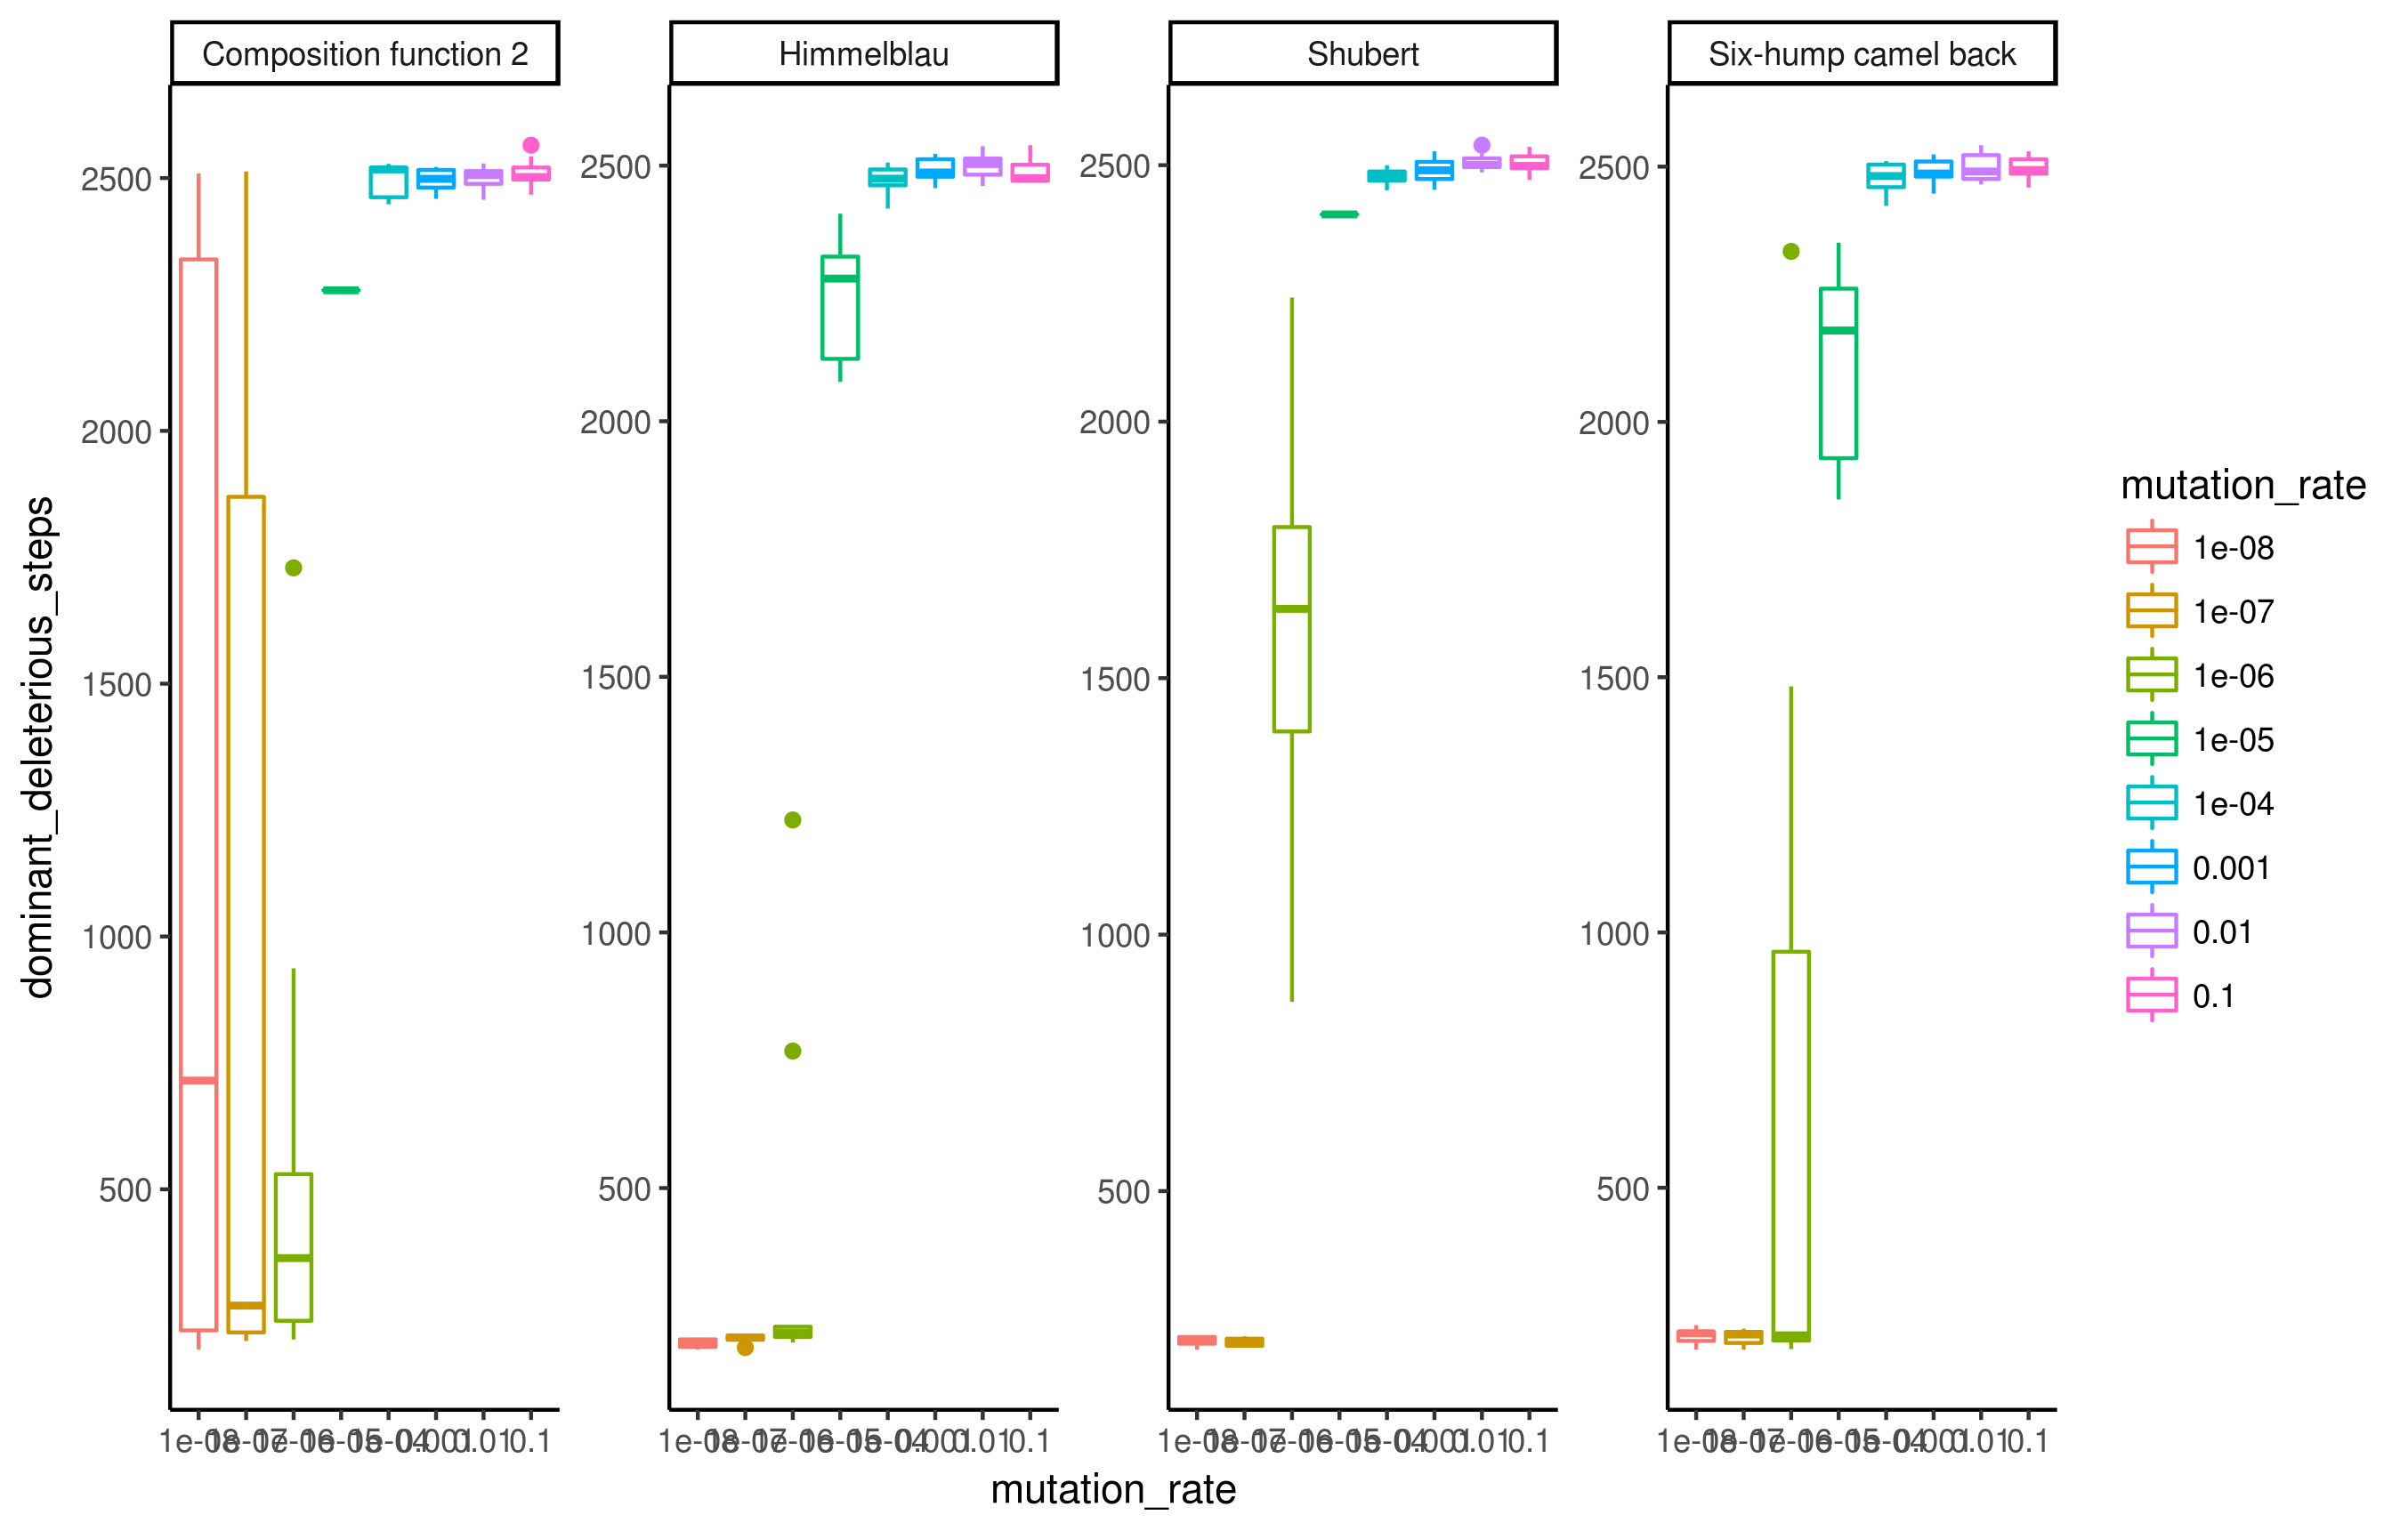
\includegraphics[width=3.5in]{figs/dom_deleterious_mutation_rate.png}
\end{figure}
\begin{figure}
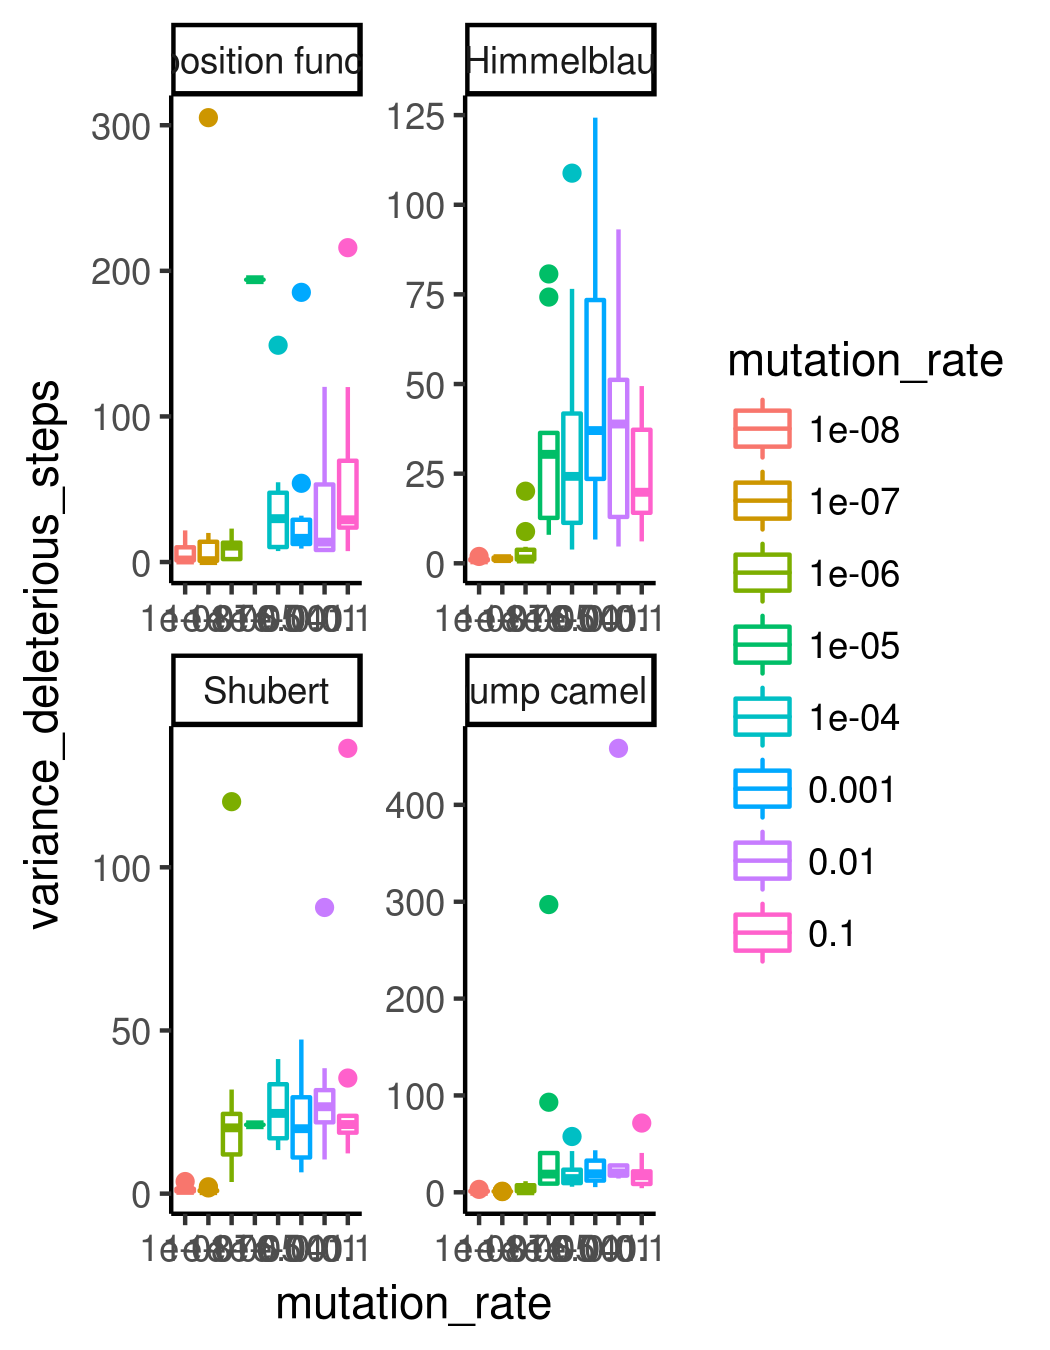
\includegraphics[width=3.5in]{figs/variance_deleterious_mutation_rate.png}
\end{figure}

% - Metric 1
% Problem 1
% Problem 2
% Problem 3
% Problem 4
% - Metric 2
% ... 

% Changing selection
% - Metric 1
% Problem 1
% Problem 2
% Problem 3
% Problem 4
% - Metric 2

\section{Conclusions}

\section{Acknowledgements}


\footnotesize
\bibliographystyle{apalike}
\bibliography{Zotero} % replace by the name of your .bib file

\end{document}
